%!TEX root = ../main.tex

\section{Preliminaries}
\label{sec:preliminaries}

\begin{figure*}[t]
    \centering
    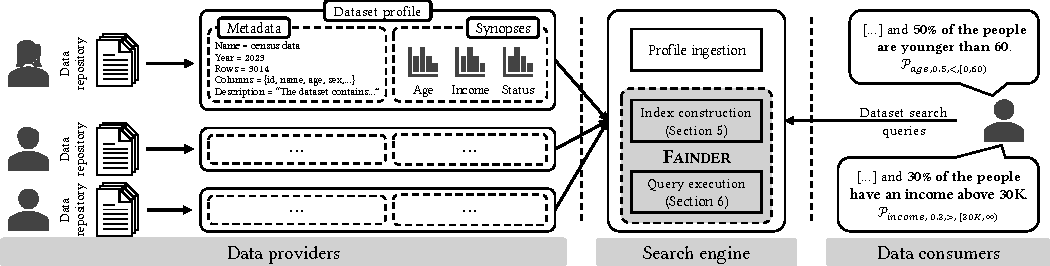
\includegraphics[scale=1]{figures/diagrams/problem_overview.pdf}
    \caption{
        Schematic overview of distribution-aware dataset search and \system{}'s role in it: Data providers offer public dataset profiles used by search engines to answer dataset search queries with distributional requirements effectively and efficiently.
    }
    \Description{Schematic overview of distribution-aware dataset search.}
    \label{fig:problem_overview}
    % Max figure width: 17.79cm
    % Max figure height: 4.5cm
    % NOTE: We place this figure here because it appears too late in the text otherwise
    \vspace{-1em}
\end{figure*}

We start by introducing basic definitions about decentralized data repositories and presenting the notation we use throughout the paper (summarized in Table~\ref{tab:notation_overview}).

\paragraph{Dataset}
A dataset is a collection of related observations organized and formatted in a particular way~\cite{chapman_dataset_2020}.
In this paper, we focus on tabular datasets that contain at least one numerical column, as they are both widespread and of particular interest when searching for datasets that meet distributional requirements.

\begin{definition}[\textsc{Tabular Dataset}]
    A tabular dataset $D$ with a schema $\cA \equiv \langle A_1,\ldots, A_l \rangle$ consists of  $l$ columns and a collection of tuples $T$ such that $t\in T$ contains $l$ values.
\end{definition}

We refer to the $i^{\text{th}}$ column of a dataset $D$ as $D[i]$.
Each dataset (and its columns) is often accompanied by specific metadata used for dataset search.
For example, Google Dataset Search~\cite{noy_google_2019} allows searching through textual dataset descriptions, while Auctus~\cite{castelo_auctus_2021} also supports search over column names and their types.
Other examples of metadata include row counts or spatiotemporal information.
We refer to these joint characteristics as dataset profiles.

\begin{definition}[\textsc{Dataset Profile}]
    A dataset profile $P_D$ is defined as the properties or constraints the tuples in $D$ satisfy.
\end{definition}

A dataset profile may contain any dataset description, such as column headers, row counts, or licenses~\cite{abedjan_profiling_2015}.
We assume that $P_D$ includes column identifiers, histograms of numerical columns, and the unit of measurement of the histogram elements.
Histograms are widely used in data management:
Database systems, such as PostgreSQL, use them for query optimization~\cite{cormode_synopses_2011}, while dataset search engines, such as Auctus~\cite{castelo_auctus_2021}, use them to visualize dataset contents.
Since data owners can decide for which columns they want to enable distribution-aware search and share histograms, we consider them a low-barrier synopsis for enriching dataset profiles.

\paragraph{Histogram}
A histogram is an approximate data synopsis that discretizes a value collection into different bins and stores the frequency of the values that fall into each bin~\cite{cormode_synopses_2011}.
Without loss of generality, we assume that histograms contain relative frequencies (i.e.,~densities) and that histogram bins are non-overlapping.

There are numerous ways to compute a histogram on top of the values in a dataset~\cite{cormode_synopses_2011}.
Our setting is agnostic to the details of histogram creation, as dataset search engines must handle a heterogeneous set of dataset profiles provided by data owners.
Consequently, we define a histogram $H_{D[i]}$ over a column $D[i]$ as a list of tuples $\langle b, v\rangle$, where bin $b \equiv [b_l, b_h)$ denotes an interval over the values in $D[i]$ and $v$ denotes the density of values in $b$.
We use \edges{$H_{D[i]}$} to refer to the list of all bin edges for the histogram $H_{D[i]}$ and \density{$H_{D[i]}$} for the corresponding list of densities.
The subscript $D[i]$ is ignored whenever it is clear from the context.

\paragraph{Data Repository}
We consider a setting where different entities (often called data providers) have their own set of datasets.
A collection of datasets $\cD=\sset{D_1,\ldots, D_k}$, gathered by one or multiple data providers, is called a data repository.
Each data repository independently computes synopses (histograms for our setting) along with other metadata of its datasets and shares them with a search engine.
To support dataset search, the search engine processes these synopses, collates a collection of histograms $\cH =\sset{H_1,\ldots, H_n}$, and evaluates user queries with it to identify relevant datasets.
